
模板还可以用来实现多态性,但不依赖基类中常见行为。相反,其共通性隐含在不同“图形”必须支持使用公共语法的操作(即,相关函数必须具有相同的名称)。具体类是彼此独立定义的(参见图18.2)。当模板用具体的类实例化时,多态功能就启用了。

\begin{center}
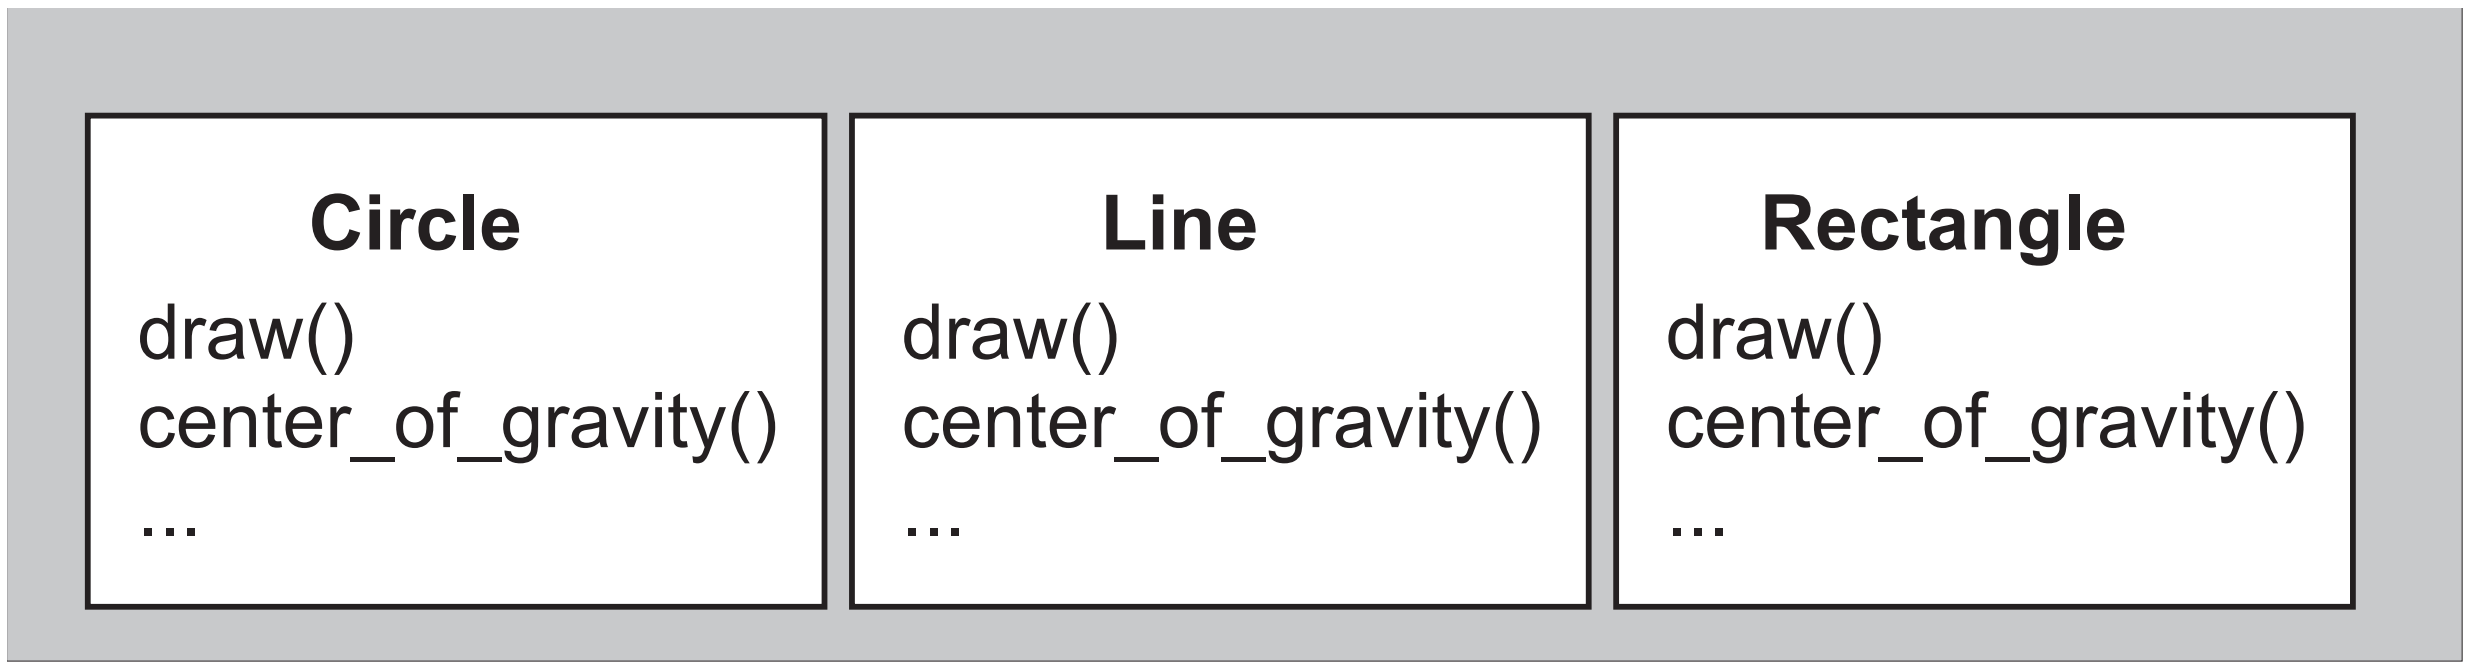
\includegraphics[width=0.8\textwidth]{content/3/chapter18/images/2.png} \\
图18.2. 通过模板实现的多态性
\end{center}

例如,前一节中的myDraw()函数:

\begin{cpp}
void myDraw (GeoObj const& obj) // GeoObj is abstract base class
{
	obj.draw();
}
\end{cpp}

可以改写为

\begin{cpp}
template<typename GeoObj>
void myDraw (GeoObj const& obj) // GeoObj is template parameter
{
	obj.draw();
}
\end{cpp}

比较myDraw()的两种实现,区别是将GeoObj规范为模板参数,而不是公共基类。然而,使用动态多态性,在运行时只有一个myDraw()函数,而对于模板有不同的函数,如myDraw<Line>()和myDraw<Circle>()。

可以尝试使用静态多态性重新写前一节的示例。首先,有几个单独的几何类,而不是几何类的层次结构:

\filename{poly/statichier.hpp}
\begin{cpp}
#include "coord.hpp"
// concrete geometric object class Circle
// - not derived from any class
class Circle {
	public:
	void draw() const;
	Coord center_of_gravity() const;
	...
};

// concrete geometric object class Line
// - not derived from any class
class Line {
	public:
	void draw() const;
	Coord center_of_gravity() const;
	...
};
...
\end{cpp}

这些类的应用如下所示:

\filename{poly/statichier.cpp}
\begin{cpp}
#include "statichier.hpp"
#include <vector>

// draw any GeoObj
template<typename GeoObj>
void myDraw (GeoObj const& obj)
{
	obj.draw(); // call draw() according to type of object
}

// compute distance of center of gravity between two GeoObjs
template<typename GeoObj1, typename GeoObj2>
Coord distance (GeoObj1 const& x1, GeoObj2 const& x2)
{
	Coord c = x1.center_of_gravity() - x2.center_of_gravity();
	return c.abs(); // return coordinates as absolute values
}

// draw homogeneous collection of GeoObjs
template<typename GeoObj>
void drawElems (std::vector<GeoObj> const& elems)
{
	for (unsigned i=0; i<elems.size(); ++i) {
		elems[i].draw(); // call draw() according to type of element
	}
}

int main()
{
	Line l;
	Circle c, c1, c2;
	
	myDraw(l); // myDraw<Line>(GeoObj&) => Line::draw()
	myDraw(c); // myDraw<Circle>(GeoObj&) => Circle::draw()
	
	distance(c1,c2); // distance<Circle,Circle>(GeoObj1&,GeoObj2&)
	distance(l,c); // distance<Line,Circle>(GeoObj1&,GeoObj2&)
	
	// std::vector<GeoObj*> coll; // ERROR: no heterogeneous collection possible
	std::vector<Line> coll; // OK: homogeneous collection possible
	coll.push_back(l); // insert line
	drawElems(coll); // draw all lines
}
\end{cpp}

与myDraw()一样,GeoObj不能再用作distance()的具体参数类型。相反,这里提供了两个模板参数GeoObj1和GeoObj2,允许在距离计算中接受不同的几何对象类型组合:

\begin{cpp}
distance(l,c); // distance<Line,Circle>(GeoObj1&,GeoObj2&)
\end{cpp}

然而,异构集合不能够透明地处理。这就是静态多态性的限制:所有类型必须在编译时确定,可以为不同的几何对象类型引入不同的集合。不再要求集合仅限于指针,因为指针仅在性能和类型安全方面具有优势。


















